\section{Nabíjení}

Aby se dveře trezoru nemusely pokaždé rozebírat kvůli nabíjení, je deska vybavena lineární nabíječkou 
\href{https://datasheet.lcsc.com/szlcsc/Seaward-Elec-SE9017-HF_C115752.pdf}{SE9017} \parencite{se9017}. 
Tento nabíjecí obvod jsem zvolil z~nabídky JLCPCB \parencite{JLCPCB} kvůli volitelnému nabíjecímu proudu, který jsem pomocí R48 \obr{fig:E4-charger} 
stanovil na 700 mA, a~také kvůli malému pouzdru a~nízké ceně.
Pro signalizaci, zda je~baterie dobita, nebo zda se ještě dobíjí, jsou zde dvě LED, LED4 a~LED5. Když se baterie dobíjí, svítí LED4, která svítí 
červeně, když je~pak baterie dobita, svítí LED5, která svítí modře.

\begin{figure}[htbp]
    \centering
    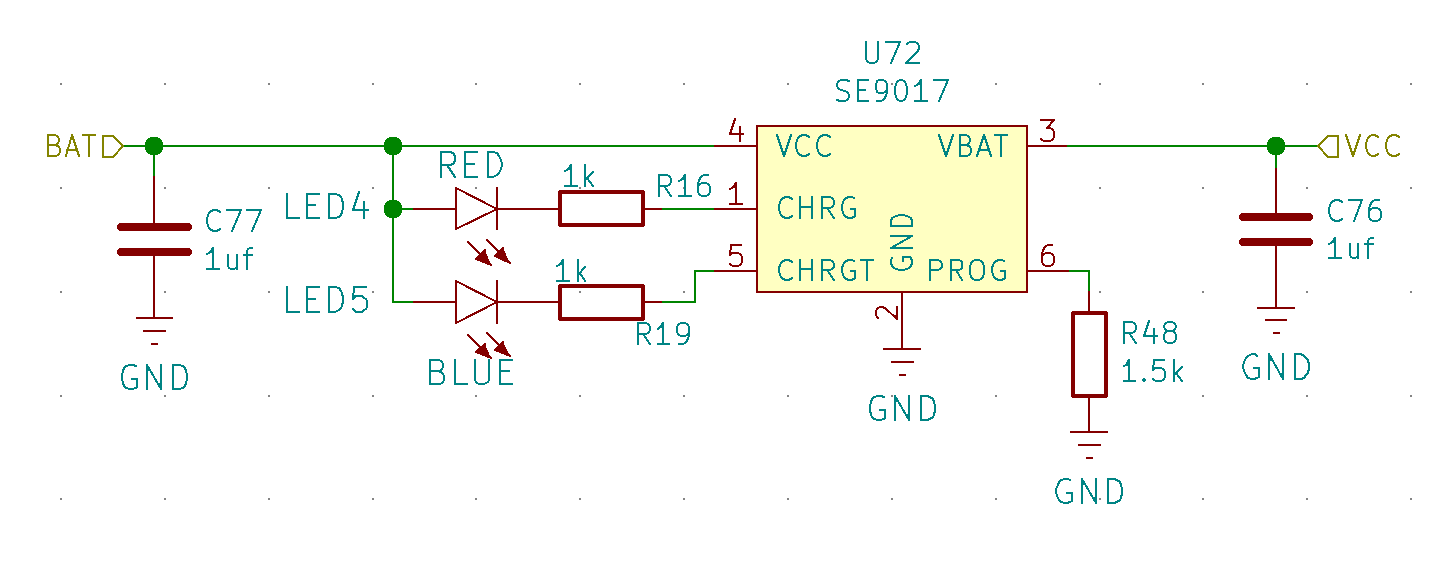
\includegraphics[width=\textwidth]{kapitoly/obrazky/E4/nabijeni/nabijecka.png}
    \caption{Zapojení nabíječky}
    \label{fig:E4-charger}
\end{figure}
